\usetikzlibrary{trees}
\tikzstyle{every node}=[draw=black,thick,anchor=west]
\tikzstyle{file}=[draw=red]
\tikzstyle{optional}=[dashed,fill=gray!20]
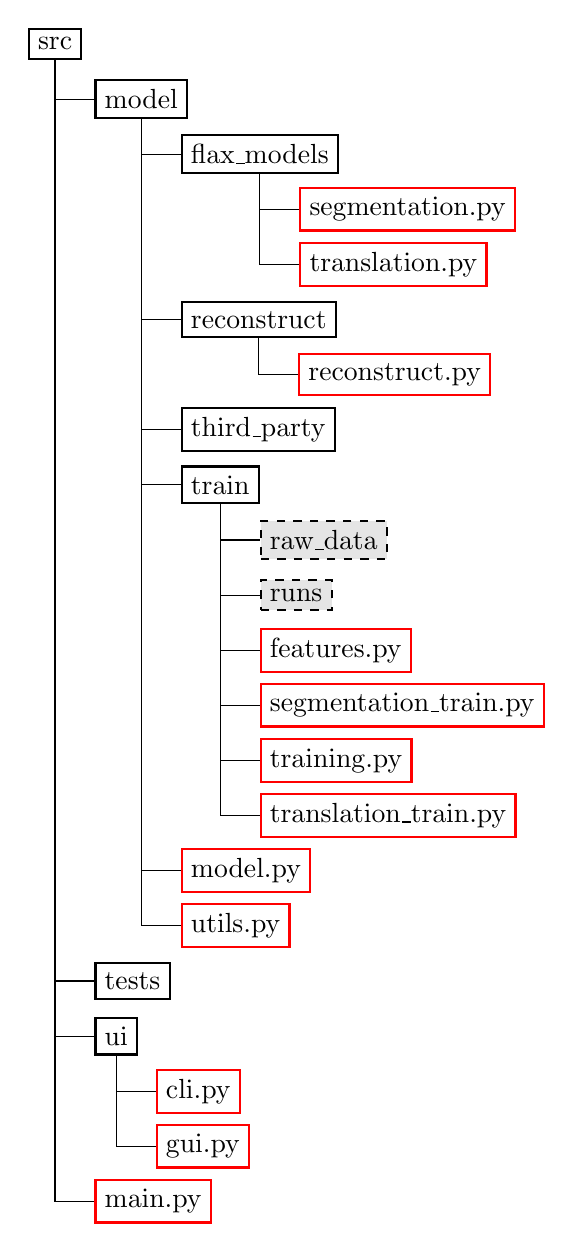
\begin{tikzpicture}[%
  grow via three points={one child at (0.5,-0.7) and
  two children at (0.5,-0.7) and (0.5,-1.4)},
  edge from parent path={(\tikzparentnode.south) |- (\tikzchildnode.west)}]
  \node {src}
    child { node {model}
      child { node {flax\_models}
        child { node [file] {segmentation.py}}
        child { node [file] {translation.py}}
      }
      child [missing] {}
      child [missing] {}
      child { node {reconstruct}
        child {node [file] {reconstruct.py}}
      }
      child [missing] {}
      child { node {third\_party}}
      child { node {train}
        child { node [optional] {raw\_data}}
        child { node [optional] {runs}}
        child { node [file] {features.py}}
        child { node [file] {segmentation\_train.py}}
        child { node [file] {training.py}}
        child { node [file] {translation\_train.py}}
      }
      child [missing] {}
      child [missing] {}
      child [missing] {}
      child [missing] {}
      child [missing] {}
      child [missing] {}
      child { node [file] {model.py}}
      child { node [file] {utils.py}}
    }
    child [missing] {}				
    child [missing] {}				
    child [missing] {}
    child [missing] {}
    child [missing] {}
    child [missing] {}
    child [missing] {}
    child [missing] {}
    child [missing] {}
    child [missing] {}
    child [missing] {}
    child [missing] {}
    child [missing] {}
    child [missing] {}
    child [missing] {}
    child { node {tests}}
    child { node {ui}
      child {node [file] {cli.py}}
      child {node [file] {gui.py}}
    }
    child [missing] {}
    child [missing] {}
    child { node [file] {main.py}};
\end{tikzpicture}